\documentclass[12pt,a4paper]{article}
\usepackage[utf8]{inputenc}

\usepackage{mathtools}
\usepackage{amsmath}
\usepackage{amssymb}
\usepackage{amsthm}
\usepackage{amssymb}
\usepackage{mathdots}
\usepackage[pdftex]{graphicx}
\usepackage{fancyhdr}
\usepackage[margin=1in]{geometry}
\usepackage{multicol}
\usepackage{bm}
\usepackage{listings}
\usepackage{xcolor}
\usepackage{pdfpages}
\usepackage{algpseudocode}
\usepackage{tikz}
\usepackage{ulem}
\usepackage{enumitem}
\usepackage[T1]{fontenc}
\usepackage{inconsolata}
\usepackage{framed}
\usepackage{wasysym}
\usepackage[thinlines]{easytable}
\usepackage{hyperref}
\usepackage{minted}
\usemintedstyle{perldoc}
\hypersetup{
    colorlinks=true,
    linkcolor=blue,
    filecolor=magenta,      
    urlcolor=blue,
}
\definecolor{codegreen}{rgb}{0,0.6,0}
\definecolor{codegray}{rgb}{0.5,0.5,0.5}
\definecolor{codepurple}{rgb}{0.58,0,0.82}
\definecolor{backcolour}{rgb}{0.95,0.95,0.92}
\lstdefinestyle{mystyle}{
    backgroundcolor=\color{backcolour},   
    commentstyle=\color{codegreen},
    keywordstyle=\color{magenta},
    numberstyle=\tiny\color{codegray},
    stringstyle=\color{codepurple},
    basicstyle=\ttfamily,
    breakatwhitespace=false,         
    breaklines=true,                 
    captionpos=b,                    
    keepspaces=true,                 
    numbers=left,                    
    numbersep=5pt,                  
    showspaces=false,                
    showstringspaces=false,
    showtabs=false,                  
    tabsize=4
}
\lstset{style=mystyle}
\newcommand\numberthis{\addtocounter{equation}{1}\tag{\theequation}}
\newcommand{\rightqed}{
\begin{flushright}
$\blacksquare$
\end{flushright}
}
\newcommand\redsout{\bgroup\markoverwith{\textcolor{red}{\rule[0.5ex]{2pt}{0.4pt}}}\ULon}
\newcommand{\solution}{\noindent\textbf{Solution:}\\\indent}
\usepackage{graphics}
\usepackage{subfig}
\graphicspath{ {./images/} }

\title{CSCI 6470 Algorithms Homework 5}
\author{Kushajveer Singh}
\date{}

\begin{document}
\maketitle

\subsection*{Problem 1}
\solution
The following logic is used to solve the MST problem using $ALGO_{MSTD}$ as a blackbox subroutine

\begin{lstlisting}[mathescape=true]
MST(G, w)
    W = sum of all weights in 'w'
    for m = 1 to W
        decision = $ALGO_{MSTD}$(G, w, m)
        if decision = Yes
            M = m
            break (from for loop)
    
    edges = []
    while True
        $G' = G - \{(u,v)\}$ (remove an arbitrary edge)
        decision = $ALGO_{MSTD}$(G', w, M)
        if decision = Yes
            G = G'
        else
            Add (u,v) to edges
        
        if number of edges in 'edges' = |V|-1
            return edges
\end{lstlisting}

\subsection*{Problem 2}
\solution
Spanning Tree = \{(G,w,M): G has a spanning tree with weight $\leq$ M\}

\newpage
\subsection*{Problem 3}
\solution
\begin{lstlisting}[mathescape=true]
Algorithm MSTD (G, w, M)
    W = 0; n = |V|
    edges = []
    for k = 1 to n-1
        nondeterministically choose $e\in E$
        add edge 'e' to edges
        W = W + w(e)
    
    G' = (V, edges)
    Use DFS to check if G' is connected
    if G' is connected and W $\leq$ M
        return Yes
    else
        return No
\end{lstlisting}

Running time of above algorithm is as follows
\begin{itemize}
    \item Line 2-3: constant
    \item Line 4: O(|E|)
    \item Line 5-7: constant. Overall Lines 4-7 run in O(|E|) time
    \item Line 9: constant
    \item Line 10: O(|V|+|E|)
    \item Line 11-14: constant
\end{itemize}

Therefore, the above algorithm is a nondeterministic polynomial-time algorithm for the decision problem MSTD.

\newpage
\subsection*{Problem 4}
\solution
The decision problem $MSTD$ has a det. p-time algorithm $A$, such that, for every input x, $x \in MSTD \iff \exists y\ A(x,y) = Yes$

\begin{itemize}
    \item For $MSTD$, input $x = (G, w, M)$
    \item Certificate for the problem is a (n-1)-edge permutation $y = \{e_1, e_2, \hdots, e_{n-1}\}$ encoding the minimum spanning tree of G
    \item We construct a verifier $A(x,y)$ that works as follows
    \begin{enumerate}
        \item $A$ checks if $y$ is a valid permutation encoding a minimum spanning tree (e.g. using DFS to check if graph is connected)
        \item $A$ checks if the total weight of the encoded tree has weight $\leq$ M
        \item $A$ output $YES$ iff it validates (1) and (2)
    \end{enumerate}
    \item $A(x,y)$ outputs $YES$ iff the given certificate $y$ encoded a minimum spanning tree with weight $\leq$ M
    \item Because $|y| = O(n)$, steps (1)-(3) can be done in $O(n)$ steps
    \item We have shown that $A$ is det. p-time verifier for $MSTD$
\end{itemize}

\subsection*{Problem 5}
\solution
$R(\phi) = \langle G_{\phi}, 4\rangle$, and $G_{\phi}$ is shown below

\begin{figure}[H]
    \centering
    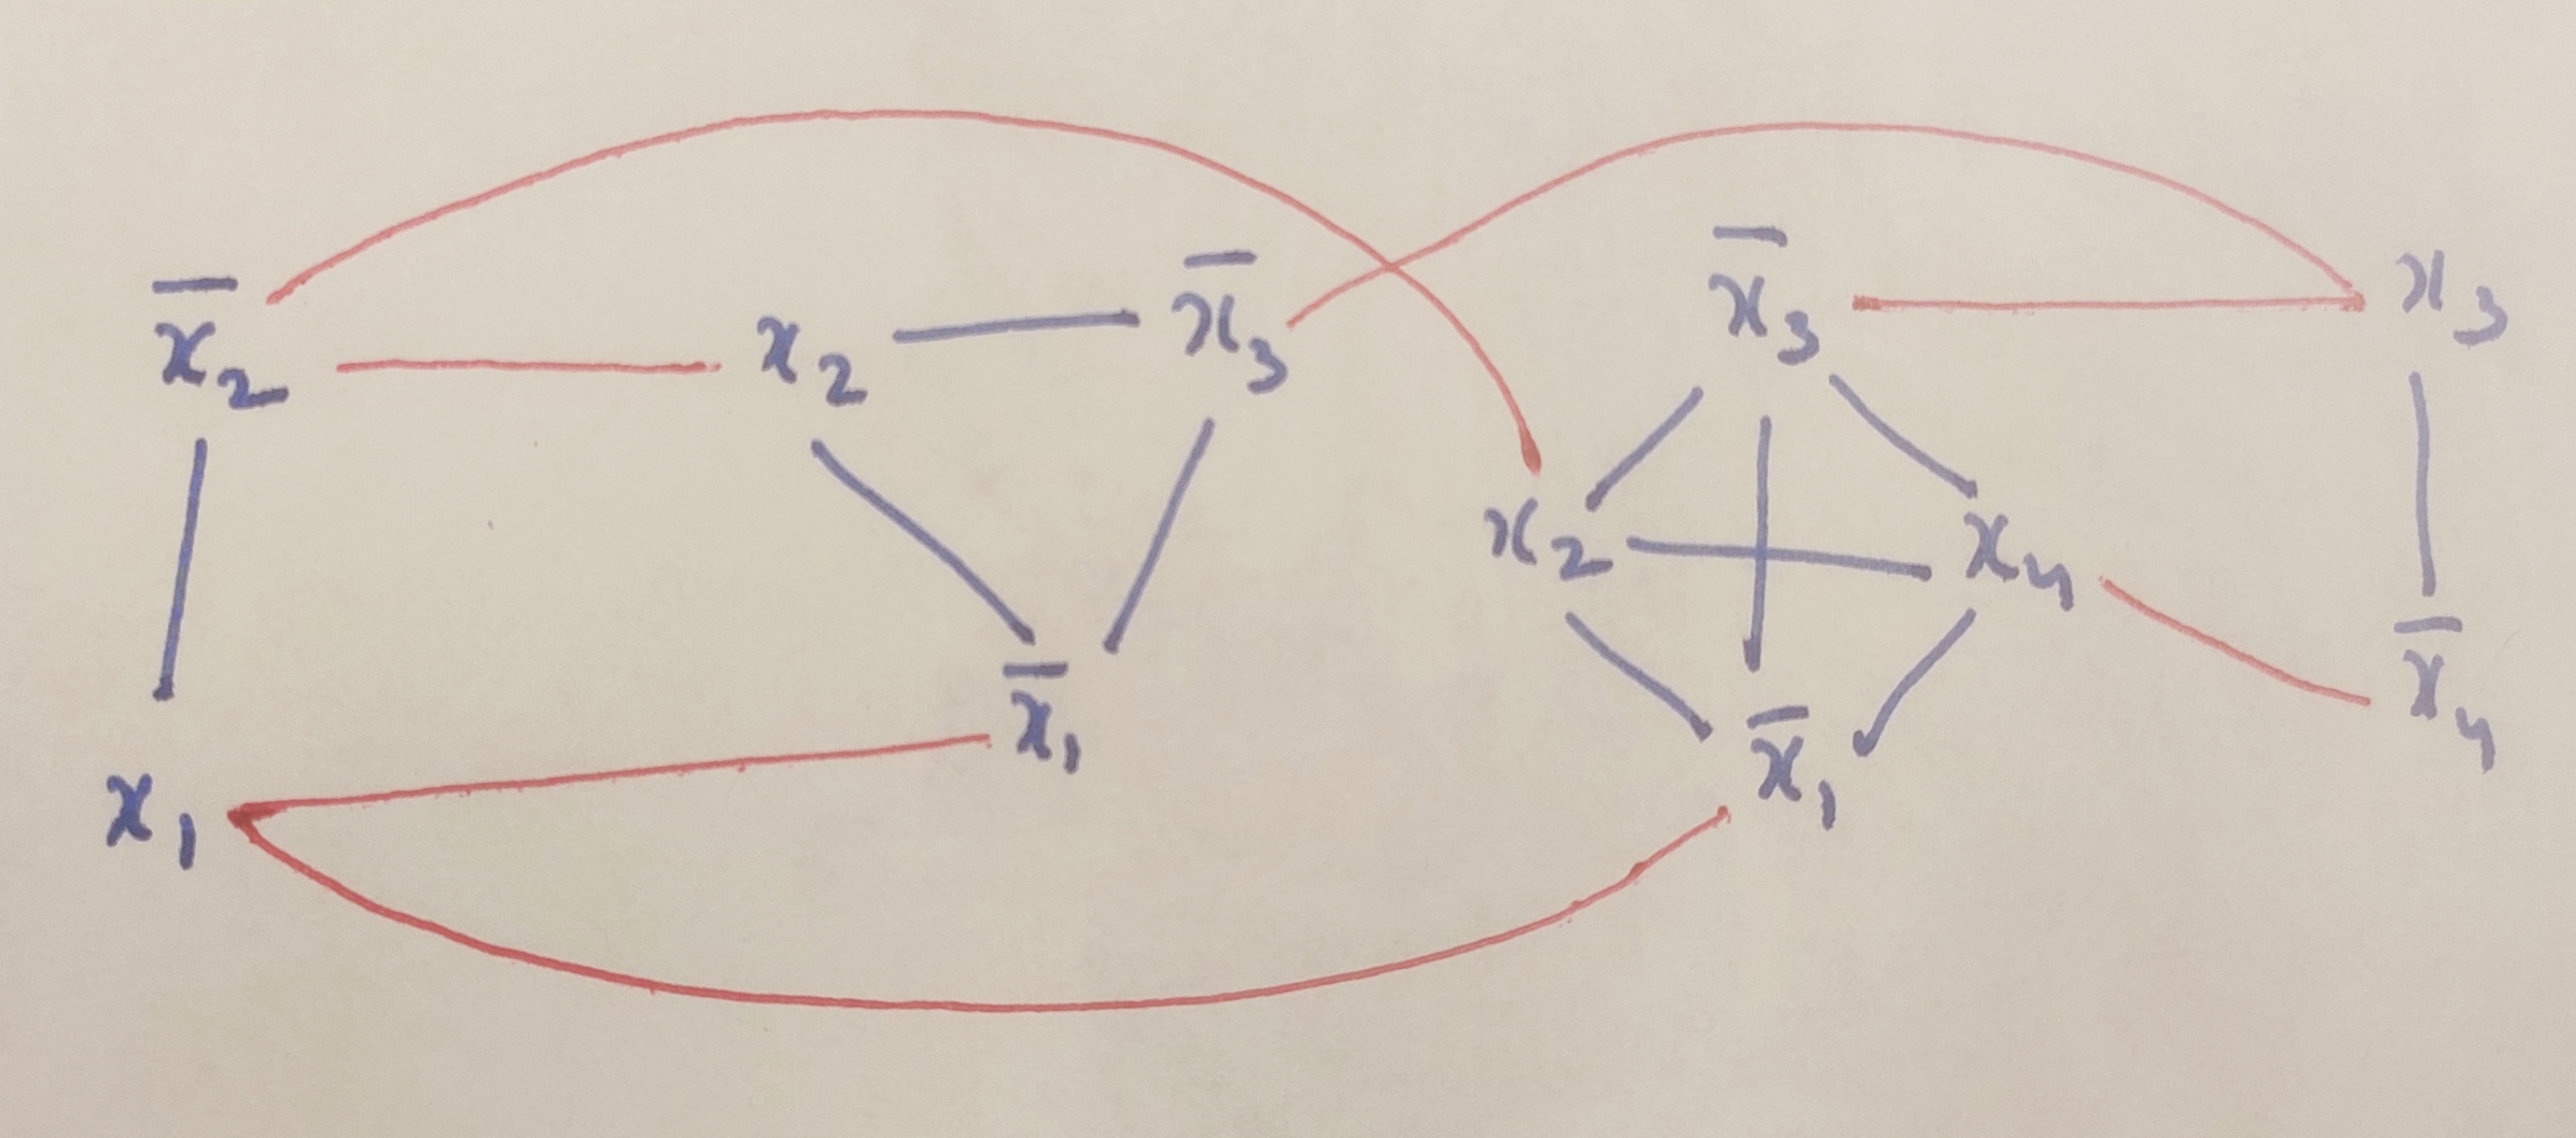
\includegraphics[width=15cm]{5.jpg}
\end{figure}

\newpage
\subsection*{Problem 6(1)}
\solution
SAT $\leq_p$ Independent Set

Using the reduction introduced in class i.e. $R(\phi) = \langle G_{\phi}, k\rangle$
\begin{enumerate}
    \item Prove $\phi \in$ SAT iff $\langle G_{\phi}, k\rangle \in$ Independent Set
    \item Prove that the reduction can be done in polynomial time in $|\phi|$ 
\end{enumerate}
The complete proof for above is in LectureNotes and we are permitted to directly use theorems from LectureNote. \\

Independent Set $\leq_p$ SAT

Using the notation introduced in class i.e. $R(\langle G_{\phi},k\rangle) = \phi$
\begin{enumerate}
    \item We first prove $\langle G_{\phi},k\rangle \in$ Independent Set iff $\phi \in$ SAT
    \begin{itemize}
        \item If $\langle G_{\phi},k\rangle \in$ Independent Set, then $G_{\phi}$ has an independent set of size $k$, which implies $\phi$ is satisfiable i.e. $\phi \in$ SAT (from slide 137 of LectureNote7+).
    \end{itemize}
    \item Now we prove that the reduction can be done in polynomial time in $|\phi|$.
    \begin{itemize}
        \item If there are $|\phi|$ number of vertices in $G_{\phi}$ then every clique would have $|\phi|/k$ on average
        \item We need to add $|\phi|/k$ vertices to the formula $\phi$, which can be done in $O(|\phi|)$.
        \item There are k cliques, so the total time for the reduction becomes $O(k|\phi|)$
        \item therefore, $R$ can be done in polynomial time in $|\phi|$
    \end{itemize}
\end{enumerate}

\subsection*{Problem 6(2)}
\solution
If we pick a decision problem $B$ and we prove $A \leq_p B$ where $A \in$ NP-hard. This means $A$ can be reduced to $B$ in polynomial time. But we also know that reduction cannot reduce the time complexity of the problem i.e. a NP-hard problem cannot be reduced to NP (because we do not know if $P = NP$). This is inferred from slide 174 of LectureNode7+ (where NP-hard problems fall outside the universe of NP problems).

So this implies that $B$ cannot be NP, which means it is NP-hard.

\subsection*{Problem 6(3)}
\solution
If $C \in P$ and $A \in$ NP-hard and $A \leq_p C$. Now consider $B \in NP$, then $B \leq_p A$.

By transitivity of mappings, we come to the conclusion that $B \leq_p C$. This means that the answer to $C$ can also be used to answer for $B$. We get a contradiction here, as we assumed that the problems in set NP are intractable (i.e. set $P$ is contained in set $NP$), so our assumption is incorrect and this proves that $NP = P$.
\end{document}
